\section{Einleitung}

\section{Methoden}
\subsection{Das dynamischer Kalman Filter}
Eicker:\\
Ein Kalman Filter findet dort Anwendung, wo bestimmte Sensoren nicht funktionieren oder sogar ausfallen und man dennoch die Systemgr��en  sch�tzen m�chte. Daf�r setzt sich das dynamische Kalman Filter aus einem Beobachtungsmodell und einem Bewegungsmodell zusammen. Bei dem Beobachtungsmodell handelt es sich um Beobachtungen und ihre Unsicherheiten. Bei dem Bewegungsmodell spricht wird auch von einer Pr�diktion (dynamisches Modell) und ihren Unsicherheiten gesprochen. Aus ihr erfolgt dann die Sch�tzung des Zustandes. 

\subsubsection{Diskreter Kalman-Filter (lineares Modell)}
Bei dem diskreten Kalman-Filter ist die Idee die Beobachtungen zu bestimmten (diskreten) Zeitpunkten mit einem Bewegungsmodell zu kombinieren. Das Bewegungsmodell pr�diziert dann den Zustandsvektor ausgehend von der Sch�tzung des vorherigen Schrittes. Generell werden vier Schritte ben�tigt: die Pr�diktion, die Innovation, die Kalman-Gain-Matrix und das Update. 

Das generelle Beobachtungsmodell sieht wie folgt aus:
\begin{equation}
\boldsymbol{l}_{i+1} = \boldsymbol{A}_{i+1}\boldsymbol{x}_{i+1} + \boldsymbol{e}_{i+1} \text{,}
\end{equation}
mit $\boldsymbol{l}$ = Beobachtungen/Messungen, $\boldsymbol{A}$ = Designmatrix, $\boldsymbol{x}$ = unbekannte Parameter und $\boldsymbol{e}$ = Residuen (Beobachtungsrauschen). Die Designmatrix beinhaltet die partiellen Ableitungen der Beobachtungsgleichungen nach den Parametern. Bei den Residuen handelt es sich um die negierten Verbesserungen. Sie sind normalverteilt mit einem Erwartungswert von 0. 

Das hier verwendete Bewegungsmodell sieht wie folgt aus:\\
\begin{equation}\label{x_i+1_allg}
\boldsymbol{x}_{i+1} = \boldsymbol{T}_i\boldsymbol{x}_i + \boldsymbol{C}_i\boldsymbol{w}_i \text{,}
\end{equation}
mit $\boldsymbol{T}$ = Transitionsmatrix (pr�diziert Bewegung von einem zum n�chsten Zeitpunkt), $\boldsymbol{w}$ = St�rgr��e (Unsicherheit im Bewegungsmodell: Rauschen), $\boldsymbol{C}$ = St�rgr��enmatrix (Auswirkung dieser Unsicherheit auf die Pr�diktion des Zustandes). Da wir annehmen, dass die Unsicherheiten im Bewegungsmodell ausreichend von den Varianzen der gesch�tzten Parameter abgedeckt werden, wird die Formel \ref{x_i+1_allg} durch die folgende Formeln ersetzt:
\begin{equation}\label{x_i+1}
	x_{i+1} = T_ix_i \text{,}
\end{equation}

St�rgr��e normalverteilt, Erwartungswert = 0 -> beeinflusst nur das stochastisches Modell aber nicht die eigentliche Pr�diktion\\

1. Pr�diktion: \\
Welche Trajektorie des Fahrzeugs sagt das Bewegungsmodell voraus?\\
$\bar{x}_{i+1} = T_i + \hat{x}_{i}$\\
$\sum(\bar{x}_{i+1}) = T_i\sum(\hat{x}_{i})T_i^T + C_i\sum(w_{i})C_i^T$\\

2. Innovation:\\
Welche Trajektorie des Fahrzeugs sagt das Bewegungsmodell voraus? Was behaupten die Beobachtungen? Wie sehr weichen die Beobachtungen von der Pr�diktion ab? => Innovation\\
$d_{i+1} = l_{+1} - A_{i+1}\bar{x}_{i+1}$\\
$\sum(d_{i+1}) = \sum(l_{i+1}) + A_{i+1}\sum(\bar{x}_{i+1})A_{i+1}^T$

3. Gain Matrix (K-Matrix):\\
Relative Gewichtung von Pr�diktion und Beobachtungen anhand der jeweiligen Genauigkeiten\\
$K_{i+1} = \sum(\bar{x}_{i+1})A_{i+1}^T\sum^{-1}(d_{i+1})$

4. Update: \\
Gewichtetes Mittel aus Pr�diktion und  Innovation\\
$\hat{x}_{i+1} = \bar{x}_{i+1} + K_{i+1}d_{i+1}$\\
$\sum(\hat{x}_{i+1}) = [I-K_{i+1}A_{i+1}]\sum(\bar{x}_{i+1})$

Geschichte des Kalman-Filters:\\
Erdunfen von Rudolf E. Kalman (Transcations of the ASME-Journal of Basic Engineering, 82 (Series D): 35-45.Copyright \copy 1960 by ASME)

Gut geeignet, um die Bahnen von Raketen zu berechnen (der Apollo Mondmission)

Dynamisches Modell: Trajektorie der Mondrakete
Beobachtungen: Space sextant, inertial navigator (Weltraumsextant, Tr�gheitsnavigator)

\subsubsection{Extended Kalmanfilter (nicht- lineares Modell)}
Weder Bewegungsmodell noch das Beobachtungsmodell ist linear, deshalb wird das extended Kalman Filter gebraucht.\\
$x_{i+1} = f^{i+1}_i (x_i, w_i)$\\
$l_{i+1} = a_{i+1}(x_{i+1}) + e_{i+1}$\\

Bei nicht-linearen Zusammenh�ngen werden die Matrizen A, T und C durch Linearisierung (partielle Ableitungen) der nicht-linearen Funktionen f und a bestimmt:

\begin{equation}
\boldsymbol{T} = \frac{\partial f(x,w)}{\partial x}
\end{equation}

\begin{equation}
\boldsymbol{C} = \frac{\partial f(x,w)}{\partial w}
\end{equation}

\begin{equation}
\boldsymbol {A }= \frac{\partial a(x)}{\partial x}
\end{equation}

Input: \\
$x_{i+1} = f^{i+1}_i (x_i, w_i)$\\

\subsubsection{Weitere Quellen:}
https://www.cbcity.de/das-kalman-filter-einfach-erklaert-teil-2

\subsection{Weigted Least-Square}
Weighted Least-Square basiert auf der Grundlage der Methode der kleinsten Quadrate. Dabei werden die Parameter so gew�hlt, dass die Quadratsumme der Verbesserungen m�glichst klein ist. 

\begin{equation}
 \left| \boldsymbol{v} \right|^2 = \sum_{i=1}^{n}v_i^2 	\rightarrow min 
\end{equation}

\begin{equation}
\boldsymbol{l}+\boldsymbol{v} = \boldsymbol{A}\boldsymbol{x} \textrm{ mit } \boldsymbol{\sum(l)} = \sigma_0^2\boldsymbol{P}^{-1}
\end{equation}

Wobei die linke Gleichung das funktionale Modell repr�sentiert, in dem der funktionale Zusammenhang zwischen Beobachtungen und Unbekannten steckt. Die rechte Gleichung nennt sich auch das stochastische Modell und dient der Beschreibung der Messunsicherheit bzw. zur Einf�hrung von Gewichten f�r die Beobachtungen. Daf�r wird die Gewichtsmatrix $\boldsymbol{P}$ eingef�hrt. 

Sch�tzung der unbekannten Parameter:
\begin{equation}
	\hat{\boldsymbol{x}} = \left(\boldsymbol{A}^T\boldsymbol{P}\boldsymbol{A}\right)^{-1}\boldsymbol{A}^T\boldsymbol{P}\boldsymbol{l}
\end{equation}

\begin{figure}[h]
	\centering
	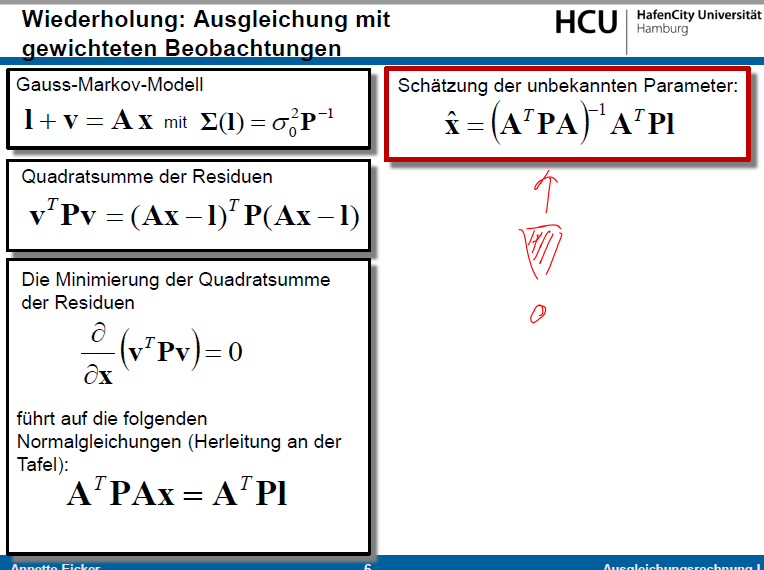
\includegraphics[width=0.7\linewidth]{source/images/GMM}
	\caption{}
	\label{fig:gmm}
\end{figure}

\section{Ergebnisse}

\section{Herausforderungen}

\section{Fazit und Ausblick}

%\bibliography